\subsection{Login}

All'avvio il sito presenta una schermata di accesso, in cui gli utenti sono invitati a inserire le proprie credenziali fornite dagli amministratori (username e password) per ottenere l'accesso al \textit{sistema}\textsubscript{\textit{G}}. Si precisa che solo gli utenti autorizzati hanno il permesso di accedere al \textit{servizio}\textsubscript{\textit{G}}. Dopo aver compilato correttamente i campi richiesti, l'utente può procedere cliccando sul pulsante di \textit{Login}\textsubscript{\textit{G}}, il quale lo reindirizzerà alla \textit{dashboard}\textsubscript{\textit{G}} principale del \textit{sistema}\textsubscript{\textit{G}}. \\
\begin{figure}[H]
    \centering
    \fbox{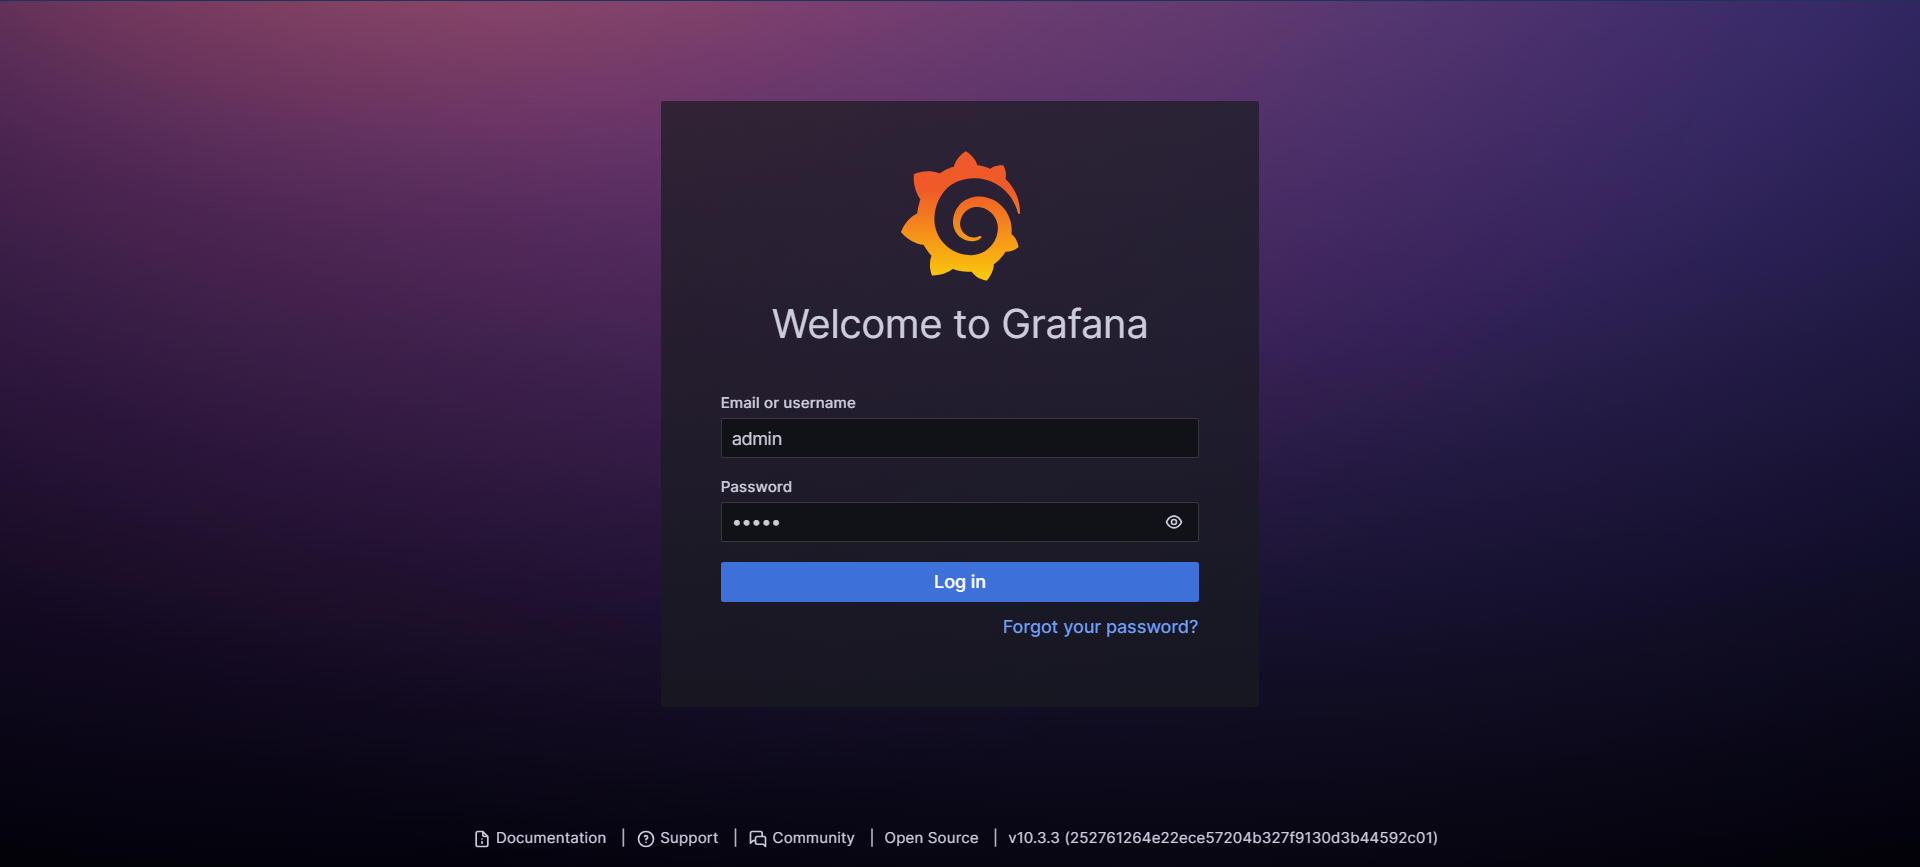
\includegraphics[width=13cm]{../Images/ManualeUtente/login.png}}
    \caption{Schermata di accesso al sistema}
    \label{fig:my_label}
\end{figure}
Nel caso in cui le credenziali siano errate, il \textit{sistema}\textsubscript{\textit{G}} mostrerà un messaggio di errore all’utente:\\
\begin{figure}[H]
    \centering
    \fbox{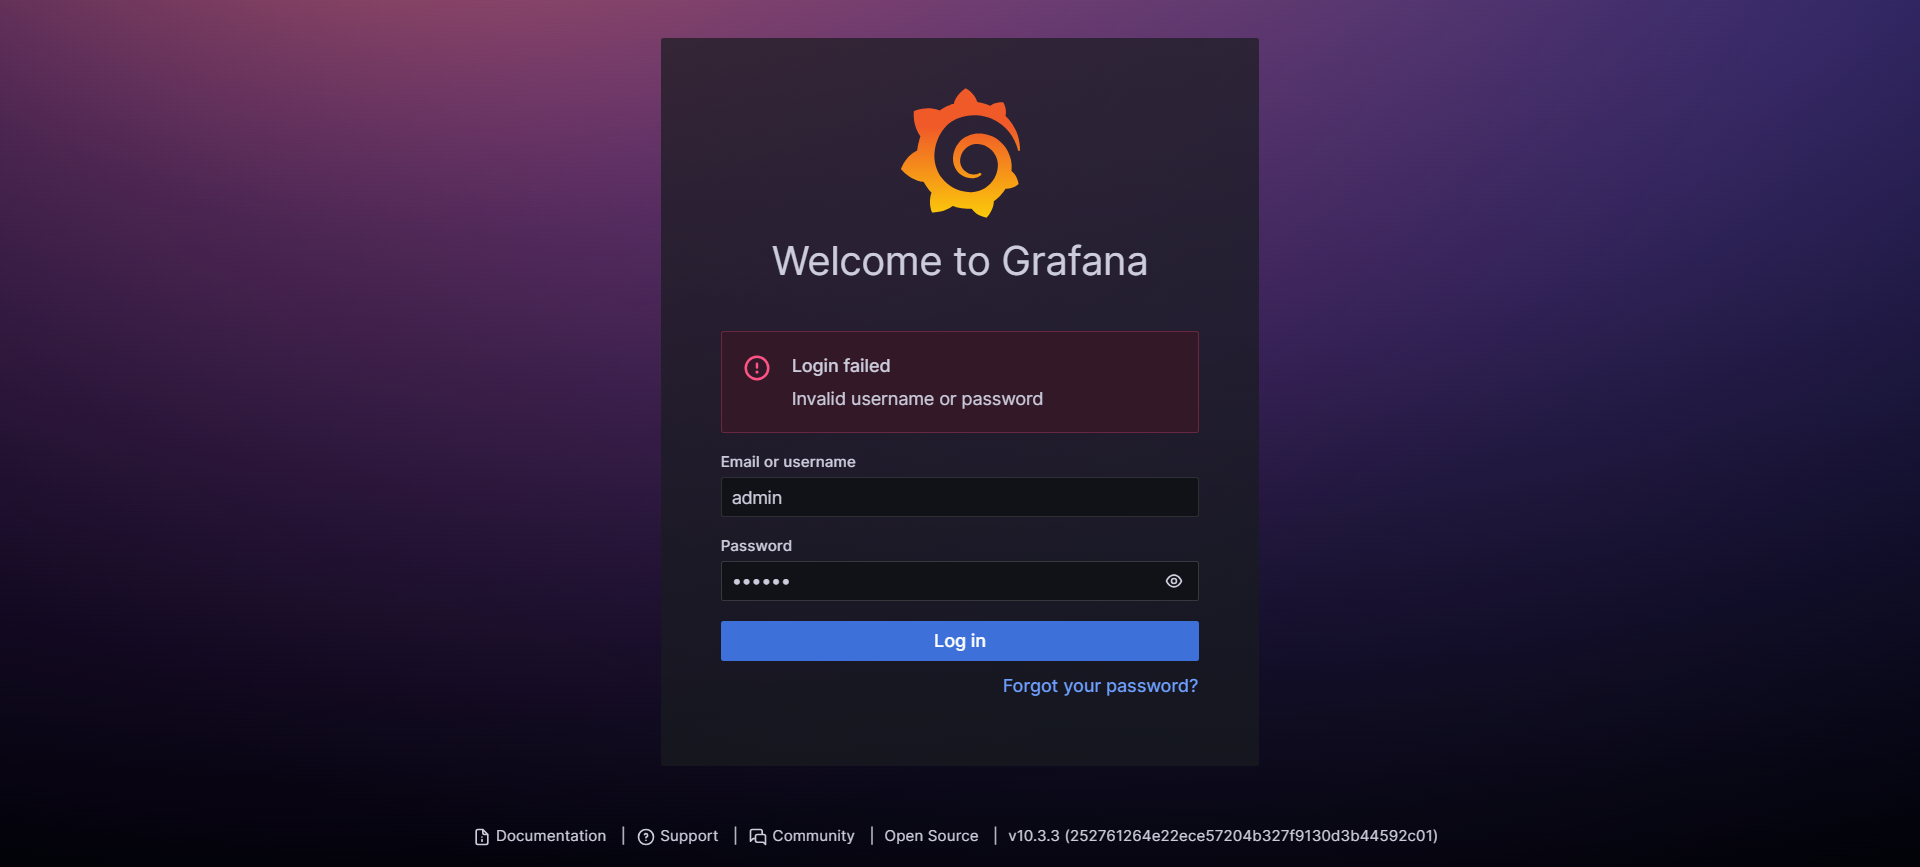
\includegraphics[width=13cm]{../Images/ManualeUtente/login-error-username_wide.png}}
    \caption{Messaggio di errore per username errato}
    \label{fig:my_label}
\end{figure}